\section{原子假说}

\begin{quotation}
“一尺之棰,日取其半,万世不竭。” \qquad 《庄子·杂篇·天下第三十三》
\end{quotation}


“原子”(atom)是物理学中的核心概念,费曼(R. P. Feynman,
1918-1988)甚至称其为物理学中最重要的概念\footnote{参考:
《费曼物理学讲义》卷I, 开篇; "If, in some cataclysm, all of scientific knowledge were to be
destroyed, and only one sentence passed on to the next generation of
creatures, what statement would contain the most information in the
fewest words? I believe it is the atomic  hypothesis that all things
are made of atoms-\emph{little particles that move around in
perpetual motion, attracting each other when they are a little
distance apart, but repelling upon being squeezed into one another}.
In that one sentence, you will see, there is an enormous amount of
information about the world, if just a little imagination and
thinking are applied.
"}。

\index{atom: 原子}

费曼假设因为某种灾难, 人类所有的知识都被毁灭了,
假如我们有机会告诉未来的文明一句话, 用最少的词汇传达最多的信息,
费曼的选择是“原子假说”(Atomic Hypothesis).
费曼以此来强调原子概念在物理学中的重要地位,
但我们知道原子假说早在2000多年前的古希腊就被当时的哲学家们提出了,
实际上原子是一个很古老的概念, 也不仅仅出现在古希腊哲学中,
如在印度哲学中有“极微说”。

\subsection{古希腊原子论}

古希腊原子论包含两个要点,首先存在原子,绝对的坚实和不可入,对应“有”,
并且存在不可分割的最小单元,原子一词在古希腊语中就是不可分割(indivisible)的意思。
其次存在虚空,虚空与原子相对,但它不可理解为“无”,而应理解为绝对的可入,绝对的可以容纳,
虚空使原子相互分离,
并提供了原子运动的舞台。原子和虚空是非常重要的概念,
它们不仅仅导向关于物性的科学, 如化学, 原子物理等; 还导向运动学,
“原子在虚空中的运动”在笛卡尔之后将被进一步理解为“质点在笛卡尔坐标系中的运动”。

原子论被后人认为是古希腊自然哲学的巅峰\footnote{关于古希腊的自然哲学与原子论,
可参考:海森堡(W. Heisenberg), 《物理学与哲学》, 第四章, 第25页;},
所谓自然哲学就是由自然出发, 用语言和逻辑去解释万事万物,
而不是通过神灵鬼怪的方式。泰勒斯(Thales,
生活于585BC)是这个传统的开始, 他一般也被认为是古希腊的第一位哲学家.
泰勒斯认为万物都可归为水。 恩培多克勒(Empedocles,
492BC-432BC)提出了水、火、土、气“四元素说”\footnote{与之类似佛教的物质论,
有所谓四大种“坚湿暖动”. 四元素和四大种很类似,
甚至我们可以直接建立: “坚即土, 湿即水, 暖即火, 动即气”这样的联系.
},后来又补充了以太, 作为构成天体和精神的第五元素。
为了解释世界的复杂和多样性,阿那克萨哥拉(Anaxagoras,
生活于500BC-428BC)提出了种子说,
即存在无数种元素,称之为种子,种子很小,小到感觉无法直接感觉到,只能通过理性把握。
面包里有肉的种子、血的种子和骨的种子,人吃了面包就能长身体,面包的种子就变成了人身体的结构。
种子说可看作是元素说的发展,只不过元素的种类变得无穷多了。

最早提出原子说的是留基伯(Leucippus,约 480 BC-约 420
BC),留基伯与阿那克萨哥拉同时代,原子说也可以看作是一种特殊的元素说,
只不过留基伯提出的元素是两种: 原子和虚空。 他认为:
“事物数目无限,它们总是相互转化。当原子坠入虚空并彼此交织时,世界就形成了。”
德谟克利特(Democritus,约 460 BC - 约 370
BC)是留基伯的学生,他认为原子可按照形状、大小进行分类,
而形状一词在古希腊语中与柏拉图的理念(idea)相同,
其实柏拉图的理念就是形状,但它强调那是理性而非感官能够把握的形,
用今天的话说就是“数学-几何学”。
柏拉图认为德谟克利特的原子说是他理念说的危险对手,
他甚至想带着自己的门徒去烧德谟克利特的著作。

这段今天读来会觉得很八卦, 其实回到2000多年前, 这是相当真实的.
首先在当时技术条件下, 著作全靠手抄, 拷贝数是有限的,
烧书是有可能彻底完成的. 其次, 古代哲学家及其门徒是政治性的团体,
他们聚集在一起是有共同政治目的的, 各门派的哲学都是综合性的.
系统化的古希腊哲学大致可分三部分,
最基础的是逻辑和方法(柏拉图是辩证法,亚里士多德是形而上学),
在此之上是自然哲学(相当于今天的科学),
而最上面的是伦理学(和政治学). 一个成功的哲学体系由逻辑和方法出发,
能够解释各种自然现象, 最后还要应用和落实在伦理学上。
柏拉图对德谟克利特原子论的反对,
不仅仅是因为他提出了一种竞争性的自然哲学,
更是因为这种自然哲学导向了一种柏拉图反对的伦理学和政治学.
这是和今天的科学完全不同的, 今天的研究是分科的,
每个学科都有自己独立的原理和问题,
我们今天不可能因为某种政治的理由去反对某个具体科学理论.


留基伯和德谟克利特的著作在今天还是失传了,
我们只能通过其他人的转述了解他们的思想,
比如亚里士多德在《物理学》中介绍并反驳了原子论的主张,
他论证了“不可能有任何连续事物是由不可分的事物合成的,
例如线不能由点合成, 线是连续的而点是不可分的.”\footnote{亚里士多德《物理学》第6卷
($231a21-231b20$);} 亚里士多德还论证了“对不可再分的物体而言,运动是不可能的”\footnote{亚里士多德《物理学》, 第6卷
($240b20-241a15$);}。

\index{Epicurus, 341 BC - 270 BC: 伊壁鸠鲁}

伊壁鸠鲁(Epicurus,341 BC - 270
BC)继承并进一步发展了原子假说,并在此基础上推出了“快乐主义”的伦理学,
伊壁鸠鲁学派是古希腊晚期重要的哲学流派之一,伊壁鸠鲁主义一度在希腊和罗马非常流行。
罗马诗人卢克莱修(Lucretius,约99BC-约55BC)是伊壁鸠鲁主义的信徒,
他流传的唯一著作《物性论》详细介绍了伊壁鸠鲁的自然哲学,
其中相当多的篇幅叙述了伊壁鸠鲁的原子思想。
到公元三世纪,罗马帝国时代的希腊作家第欧根尼·拉尔修编撰了关于古希腊各哲学流派哲学家的传记作品《名哲言行录》,
其中第十卷是关于伊壁鸠鲁的,第欧根尼·拉尔修在其中抄录了三封伊壁鸠鲁致友人的信,
其中致希罗多德书信(Letter to Herodotus\footnote{请阅读:
《自然与快乐:伊壁鸠鲁的哲学》 })是关于原子论的。


伊壁鸠鲁对德谟克利特原子假说的主要改进是(1)提出了“原子的偏转”(swerve),
即认为原子在运动过程中的任何一点都可能发生微小的偏转,
原子的运动不再是决定性的了,
伊壁鸠鲁认为这样就避免了德谟克利特的宿命论,
为“自由意志”保留了可能\footnote{“自由意志”在基督教神学中是很重要的概念,
因为如果人的行为完全是由原子的机械运动所决定(或完全由上帝的事先安排所决定),
那么个人就无需为自己的罪恶负责了。}。
也经常有人会把德谟克利特的原子论比作牛顿和拉普拉斯的机械力学,
而把伊壁鸠鲁引入“偏转”概念的原子论比作量子力学(“偏转”对应“量子跃迁”,量子力学中的跃迁也不是决定性的,而是几率性的)。
(2)伊壁鸠鲁认为原子不可能取所有的大小, 其大小是有上限的,
因为从来没有人见过原子, 另外原子的大小也是有下限的,
即不可能是任意小的.
伊壁鸠鲁强调“除形状、大小、重量和其他必然与形状联系在一起的性质外,
不应当认为原子还具有其他属性。”这里,
原子具有形状是原子论解释物性的基础,有形状就意味着有部分,
即在想象意义或数学意义下是可分的,那么在想象意义下原子是否无限可分呢?
伊壁鸠鲁仍然主张不能无限可分,因此有想象中的极小,没有形状,但却有体积,
并可用来度量体积。如果把亚里士多德和伊壁鸠鲁的观点做个比较的话,亚里士多德反对原子,
主张在自然和数学意义下都“无限可分”,而伊壁鸠鲁则正好相反,在自然和数学意义下都主张原子论。


在整个漫长的中世纪,原子论被欧洲人遗忘,哲学与诗歌和戏剧一起被作为异教的焚烧。
柏拉图的《蒂迈欧篇》是唯一流传的自然哲学著作,十字军东征后,亚里士多德的著作开始流传,
这为原子论的复兴奠定了基础。文艺复兴时期的1417年,意大利学者布拉乔利尼(Poggio
Bracciolini)在一个修道院里重新发现了卢克莱修的《物性论》并流传给当时的知识界。
随后,蒙田(Montaigne,1533-1592)、伽森狄
(Gassendi,1592-1655)等复活了伊壁鸠鲁的原子论思想,并通过玻意尔(Boyle,1627
-
1691)、道尔顿(Dalton,1766-1844)等实验物理学家的工作逐渐发展出了关于原子的近代理论。

\subsection{近代原子论}

\subsubsection{富兰克林油膜实验}

原子是超越经验的概念, 我们无法用感官直接感觉到原子的存在,
但有了原子的概念可以帮助我们融贯地理解很多日常观察到的现象。温伯格(Steven
Weinberg, 1933-)在《亚原子粒子的发现》中举例说:
“取一些盐溶解于一碗水里, 用原子论就很容易解释这一现象:
组成盐的原子分散到水原子之间的虚空中去了 ... 再例如,
一滴油滴在水面上, 它将扩散到一定的面积后才终止扩散,
用原子论很容易解释这种现象:
薄薄的油膜一直扩散到只有几个原子的厚度的时候, 才终止扩散。”
温伯格举的两个例子都是我们的日常经验,
这些现象即便在古代都应是人们熟悉的。第一个例子是古代原子论者经常举的例子,
第二个例子就是富兰克林油膜实验。

\index{Franklin's Oil-Drop Experiment: 富兰克林油膜实验}

富兰克林(Franklin)在1773年发现当把少量橄榄油放到水面上,
油膜最大只能覆盖有限的水面。假设橄榄油是由不可再分的体积有限的“原子”组成的,
我们就能由此估算原子的尺寸。富兰克林把一勺油,大约$5 cm^3$倒入池塘,
发现大约$2000 m^2$的水面被油膜覆盖了, 由此我们可估算出油膜的厚度,
大约是$2.5 nm$, 这可算是对原子尺寸的第一次定量估计了。

\begin{equation}
 d = \frac{V}{S} = \frac{{5 \times \left( {10^{ - 2} m} \right)^3
}}{{2 \times 10^3 m^2 }} = 2.5 \times 10^{ - 9} m
\end{equation}

$2.5 \times 10^{-9} m$即2.5纳米,这和细胞膜的厚度7-8纳米在同一数量级,考虑到细胞膜是两层油膜(脂双分子层)构成的,单层就是大约3.5纳米,富兰克林的估算在定量的意义下都已经很“准确”了。

结论:油这种物质存在基本单元(即存在“油的原子”),其大小是大约2.5纳米。

\subsubsection{道尔顿的原子假说}

随着工业化和近代化学的建立,原子学说获得了本质的进展。
1803年,英国科学家道尔顿(John Dalton, 1766 -
1844)提出了近代意义上的原子论:

\index{John Dalton, 1766 - 1844: 道尔顿}

\begin{enumerate}

\item{ 原子是组成化学元素的、非常微小的、不可再分割的物质微粒。
在化学反应中原子保持其本来的性质。}

\item{ 同一种元素的所有原子的质量以及其他性质完全相同。不同元素
的原子具有不同的质量以及其他性质。原子的质量是每一种元素的原子
的最根本特征。}

\item{ 有简单数值比的元素的原子结合时,原子之间就发生化学反应
而生成化合物。化合物的原子称为复杂原子。}

\item{ 一种元素的原子与另一种元素的原子化合时,他们之间存在
简单的数值比。}

\end{enumerate}

{\bf 例1:} $2H{}_2 + O_2
\mathbin{\lower.3ex\hbox{$\buildrel\textstyle\rightarrow\over
{\smash{\leftarrow}\vphantom{_{\vbox to.5ex{\vss}}}}$}} 2H_2 O$,
两倍体积的氢气与一倍体积的氧气恰好完全反应,生成水;或:
1克氢气与8克氧气完全反应生成9克水。由此可猜想:水分子由两个氢原子,
一个氧原子构成。


\subsubsection{法拉第电解定律}


人类很早就知道了电现象, 丝绸摩擦玻璃棒带正电, 毛皮摩擦橡胶棒带负电,
这是关于静电的研究. 金属可以导电, 并导致相应物理效应,
这是所谓动电的研究. 电学的研究在19世纪达到了很高的成就,
并与更古老的学问——磁学——联系了起来,
电磁学的最后完成很大程度上可归功于法拉第和麦克斯韦两位英国科学家,
法拉第是实验物理学家,而麦克斯韦则是位理论物理学家,类似于第谷和开普勒的关系。

1833年,法拉第(Michael Faraday, 1791 -
1867)发现电解定律:电解时,在电极上析出或溶解掉的
物质的重量,与通过电极的电量成正比;如通过的电量相同,
则析出或溶解掉的不同物质的摩尔数\footnote{1摩尔(mol)
物质包含阿佛加德罗常数$N_A$个粒子。}相同。


\begin{figure}[h]
\begin{center}
  % Requires \usepackage{graphicx}
  \includegraphics[width=6cm]{AtomIdea/faradaylaw.ps}\\
  \caption{法拉第电解水实验}
\end{center}
\end{figure}


\index{Faraday's  laws of electrolysis: 法拉第电解定律}

{\bf 例2:}电解水实验,$H_2 O \rightarrow 2H^ +   + O^{2 - } $,
法拉第发现每电离出1克氢气(或8克氧气),需要96485库仑电量( 定义:$1F
= 9.6485 \times 10^4
C$)。由此我们可以猜想:1)原子中可能有“标准”带电粒子——“电子”
存在,电荷是“量子化”的;
2)电磁相互作用是原子组成分子及物质聚集(气、液、固三态)的物理原因。
如果我们知道电子的电荷,就可以计算出阿佛加德罗常数:$N_A  = F/e$。

法拉第工作的意义是把化学与物理学联系起来,成为统一的科学。


\subsection*{阅读材料}

\begin{itemize}
  \item 张竹明 译, 亚里士多德《物理学》
  
  \item 王玮玮
等译,《自然与快乐: 伊壁鸠鲁的哲学》

\end{itemize}
